\documentclass[letterpaper, 10 pt]{article}
\usepackage[spanish]{babel}
\usepackage[margin = 1 in]{geometry}
\usepackage[utf8]{inputenc}
\usepackage{graphicx}
\usepackage{hyperref}
\hypersetup{
	colorlinks=true,
	linkcolor=black,
	urlcolor=blue,
	pdftitle= Uso de Q-learning y redes neuronales como alternativa
}
\usepackage{fancyvrb}
\usepackage{fancyhdr, lastpage}
\pagestyle{fancy}
\lhead{Universidad Autónoma de Nuevo León}
\rhead{Facultad de Ingeniería Mecánica y Eléctrica}
%\cfoot{Page \thepage\ of %\pageref{LastPage}}
%\lfoot{Footnotes pages}
\rfoot{\today}
\usepackage{parskip}
\usepackage{setspace}
\onehalfspacing

\newcommand{\Tittle}[1]{ {\Huge \bfseries{ #1 }}  }
\newcommand{\subTittle}[1]{ {\Large \bfseries{ #1 }}  }
\newcommand{\normalTittle}[1]{ {\normalsize \bfseries{ #1 }}  }


\begin{document}

%\ttfamily %mecanografiada
%\rmfamily %Roman
\sffamily %sans
\begin{center}

	\Tittle{Uso de Q-learning y redes neuronales como alternativa a la solución del problema flexible scheduling} \par
	\subTittle{Arnoldo Del Toro Peña}  \par
	\subTittle{Supervisor de tesis:} \par
	\subTittle{Dr. Vincent Andre Lionel}\textbf{\Large Boyer } 
\end{center}

\begin{abstract}
	Se define una búsqueda Q-learning como alternativa a la solución de un problema Flexible Scheduling, se establecen análisis a los resultados obtenidos en contraste a resultados obtenidos por métodos metahuerísticos.
	% It's  a brief summary of approximately 300 words. It includes the important questions, the rationale for the study, the hypothesis, the method, and the other characteristics. When describing the method, the design, procedure, results, and discussion must be included.
\end{abstract}

\section*{Por favor dé una breve justificación de su proyecto de investigación propuesto:}
La gran cantidad de tesis con métodos metahuerísticos deja muchas preguntas en el aire, y nos abre el camino para tratar de explorar nuestras alternativas a estos mismos, tanto para mejorar o descartar posibles caminos.
% In this section, the research proposal must be justified.

\section*{Objetivos}
Evidenciar si es viable un método alternativo a un método metahuerístico.
% Describe clearly and concisely the objective of your research proposal.

\section*{Introducción}
% Establecer el territorio

Uno de los métodos más utilizados es el método metahuerístico, dejo en claro que no se pretende criticar nada de ellos, pero en los últimos años estos han sido demasiado utilizados, llegando a ser el ingrediente esencial al momento de intentar solucionar un problema de Optimización.

Esto representa un tema interesante al momento de pensar en alternativas a métodos metahuerísticos, lo cual nos lleva a cuestionar si el uso de estos es debido a su efectividad, rapidez o algún otro factor.

% Establecer el nicho

En este documento no se pretende verificar alguno de estos factores en los métodos metahuerísticos, si no que se pretende presentar una posible alternativa a estos mismos, tomando como partida los resultados ya obtenidos por algún método metahuerístico.

% Ocupar el nicho

Es aquí donde estableceremos nuestra atención, en una alternativa para la solución de problemas resueltos por métodos metahuerísticos.

Estableceremos una solución por medio de un aprendizaje "Q-learning" y por medio de redes neuronales nuestro agente tendrá la capacidad de resolver estos problemas, una de las características de nuestra alternativa es que el aprendizaje "Q-learning" sus tiempos tienden a un número muy grande de iteraciones el cual está en contraste con un método metahuerístico.

Posteriormente compararemos el resultado generado por el aprendizaje implementado en contraste a una solución generada por un método metahuerístico.

Por último mencionar que nos centramos  solo en el problema  Flexible Scheduling problem.

\section*{Antecedentes}
%#FIXME cambiar antecedentes a estado del arte, y en antecedentes agregar libros que tengan que ver con métodos o procesos de tu tesis
Xinwei Chen, Marlin W. Ulmer, Barrett W. Thomas, University of Iowa,se presenta los detalles de la implementación DQL, los resultados analíticos junto con pruebas, ilustraciones de la toma de decisiones, combinaciones de funciones adicionales, un análisis del valor de no ofrecer el servicio y los resultados para expandir las decisiones de asignación.


Se utilizó una estructura básica para cada una de las tres NN's: Input Layer, Hidden Layer and Output Layer.

El artículo presenta unas variables de drones, vehículos terrestres y no prestar el servicio, cada una de estas variables es analizada a lo largo del artículo.

El artículo presenta unos resultados muy favorables a las ecuaciones planteadas (`` Q-learning '' ), pero no compará sus resultados con algún método metahuerístico, en este mismo artículo se agrega un apartado donde se analizan los casos de cada una.

Un apartado interesante es en el que señalan que podría utilizarse un método metahuerístico para determinar la solución pero que este mismo limita las variables por lo cual no lo hicieron.

\section*{El estado del Arte}
Tomando en cuenta la actual literatura que tenemos, hay muchos artículos que hablan de ``Q-learning'' con redes neuronales aplicadas a la solución de problemas de ruteo, asignación, entre otras ... en general problemas de optimización, ninguno de ellos (hasta el momento) a presentado un análisis en contraste con el uso de métodos metahuerísticos, por lo cual nos motiva a seguir pero también a tener precaución, ya que queda una pregunta en el aire, ¿Será útil la comparación?

Lo que se quiere expresar es que el hecho de no haber tantos artículos puede ser debido a los carentes resultados comparados con los correspondientes de métodos metahuerísticos o por el excesivo tiempo de aprendizaje o tal vez por algún otro factor negativo hacia el aprendizaje ``Q-learning''.

\section{Literature  Review}
Sometimes the literature review is incorporated into the introduction section.
However, most professors prefer a separate section, which allows a more thorough
review of the literature.
\newline Import points:
\begin{enumerate}
	\item Organization and structure.
	\item Focus, unity, and coherence.
	\item Not be repetitive or verbose.
	\item Falling cite.
	\item Citing irrelevant or trivial references.
	\item Not depending too much on secondary sources.
\end{enumerate}

\section*{Solución propuesta y Diseño de experimentos}
La oportunidad de implementación de un algoritmo por aprendizaje automatizado, se presenta al momento de tener una cantidad exhaustiva de métodos metahuerísticos.

Las instancias se recolectaron de los artículos presentados en la bibliografía.

El objetivo de nuestro experimento es poder analizar si es realmente factible utilizar un algoritmo de aprendizaje automatizado en paralelo o en reemplazo de un método metahuerístico.

Se presentan un conjunto de instancias de medidas variadas, es importante señalar que las instancias se presentan de manera independiente.

De cada instancia se tiene el mejor resultado obtenido por medio de un proceso metahuerístico, que se detalla en cada una de las instancias (no se profundiza en el método metahuerístico).

Cada instancia se somete al algoritmo propuesto, de inicio se presentan resultados con un criterio de parada de n horas, posteriormente se presentan los resultados de la instancia con mejor aproximación sin un límite de n horas. 

El proceso no se tiene definido actualmente, aun se sigue trabajando en la ecuación para el aprendizaje por lo cual los detalles del proceso interno sigue en construcción.

En la siguiente tabla se presentan los resultados de cada instancia:

\begin{center}
	\begin{table}[ht]
		\centering
		\begin{tabular}{|c|c|l|l|}
		\hline
		\multicolumn{1}{|l|}{\textbf{Instancia}}                   & \multicolumn{1}{l|}{\textit{\begin{tabular}[c]{@{}l@{}}Resultado \\ Metahuerística\end{tabular}}} & \multicolumn{1}{c|}{\textit{\begin{tabular}[c]{@{}c@{}}Resultado\\ Algoritmo\end{tabular}}} & \multicolumn{1}{c|}{\textit{Horas}}               \\ \hline
		\textit{1}                                                 &                                                                                                   &                                                                                             & $n_1 $                                             \\ \hline
		\textit{2}                                                 &                                                                                                   &                                                                                             & $n_2$                                              \\ \hline
		\textit{\begin{tabular}[c]{@{}c@{}}.\\ .\\ .\end{tabular}} &                                                                                                   &                                                                                             & \begin{tabular}[c]{@{}l@{}}.\\ .\\ .\end{tabular} \\ \hline
		\textit{m}                                                 &                                                                                                   &                                                                                             & $n_m$                                              \\ \hline
		\end{tabular}
		\end{table}
	
\end{center}

Y en la siguiente gráfica se presentan los valores de manera discreta de los resultados en ambos métodos.

\begin{figure*}[h!t]
	\centering
	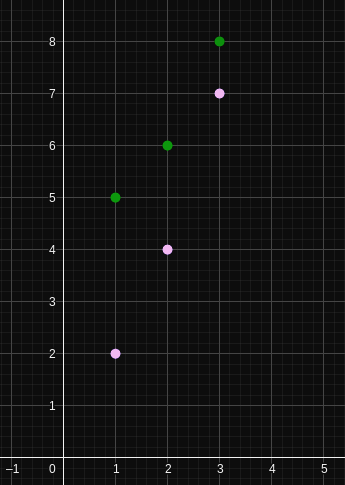
\includegraphics[scale = 0.2]{ejemplo_grafica.png}
	\caption{Ficticio}
\end{figure*}

Primero se presentan los análisis de aproximación de resultados, para ello se toman los valores de resultados, tanto de metahuerísticos como del algoritmo.

El análisis propuesto es el valor relativo, tomando como valor real el resultado obtenido por los métodos metahuerísticos.

El siguiente factor a analizar es el tiempo asignado para cada uno de las instancias en nuestro algoritmo, para ello se realiza una diferencia en valor absoluto entre las horas de nuestro algoritmo y el tiempo de ejecución de cada método metahuerístico, estos  últimos se presentan a continuación:

\begin{table}[ht]
	\centering
	\begin{tabular}{|c|c|}
	\hline
	\multicolumn{1}{|l|}{\textbf{Instancia}}                   & \multicolumn{1}{l|}{\textit{\begin{tabular}[c]{@{}l@{}}tiempo por\\ método metahuerístico\end{tabular}}} \\ \hline
	\textit{1}                                                 &                                                                                                          \\ \hline
	\textit{2}                                                 &                                                                                                          \\ \hline
	\textit{\begin{tabular}[c]{@{}c@{}}.\\ .\\ .\end{tabular}} &                                                                                                          \\ \hline
	\textit{m}                                                 &                                                                                                          \\ \hline
	\end{tabular}
	\end{table}



Ya que se presentaron los tiempos se tomamos el menor de la diferencia, la instancia que se representa esta diferencia será la que a continuación mostramos los resultados sin un tiempo de n horas. Las diferencias las podemos ver en la siguiente tabla:

Una vez que tenemos los resultados de la instancia seleccionada se presenta a continuación los análisis sobre un próximo experimento.

\begin{center}
	Insertar resultados
\end{center}

Nota: las conclusiones como la confirmación del experimento y próximos posibles experimentos dependen de los resultados obtenidos.

Aun sin tener resultados, una mejora a este experimento es asignar al algoritmo un mayor número de instancias, esto es debido a que entre más se utilice el algoritmo este mismo se vuelve más eficaz; algo que se sabe de antemano es el excesivo costo de tiempo de ejecución de un algoritmo como el que estamos proponiendo, por lo cual sabemos de antemano que si la variable de tiempo es muy importante para nuestro problema no es factible para nuestro algoritmo; sin embargo la posibilidad de en un futuro cercanos solo insertar las instancias para tener una solución de una calidad similar a un método metahuerístico es la motivación a nuestro experimento.



% \section{Methods}
% The Method section is very important because it tells your Research Committee how
% you plan to tackle your research problem. It will provide your work plan and describe
% the activities necessary for the completion of your project.
% You need to demonstrate your knowledge of alternative methods and make the case
% that your approach is the most appropriate and most valid way to address your
% research question. \newline
% For quantitative studies, the method section typically consists of the following
% sections:
% \begin{enumerate}
% 	\item Design.
% 	\item Subjects or participants.
% 	\item Instruments.
% 	\item Procedure.
% \end{enumerate}

\section{Metodología}
El diseño estará conformado de inicio, en la implementación de una búsqueda basada en Q-learning, se buscará que en lugar de guardar los resultados en una tabla (lo que es habitual en Q learning) conectaremos estos mismos a  una red neuronal y que por medio de esta misma se de el aprendizaje,después todo esto se aplicará a un problema de flexible job shop scheduling problem.

Se programará en python 3.7 por la disponibilidad en las bibliotecas encontradas. (las especificaciones del equipo están pendientes).

Aún estamos en la etapa de investigación, la cual solo ha tenido como resultados un par artículos, los cuales tendrán las respectivas referencias (este apartado hay que detallarlo más ya que los artículos aún están en revisión).

Lo primero que estamos planeando explorar es el uso de Q-learning, el cual solo hemos podido importar algunas librerías para el uso en problemas de 2-D, los cuales no son muy importantes para lo que tenemos planeado, sin embargo seguimos en la etapa de exploración.

Lo segundo que queremos es crear una pequeña red neuronal a la que también aplicaremos unas pequeñas pruebas en un problema.

Una vez que tengamos verificado el uso en cada uno de estos antes  mencionados, lo que haremos será enlazarlos de una manera que el aprendizaje (que normalmente se obtendría con una fórmula de Q-learning) ahora provenga de una red neuronal.

Si logramos esto lo siguiente será introducir unas instancias del problema clásico flexible job shop scheduling problem, en el cual existen ya demasiados resultados con el objetivo  de ver que tan precisos serian nuestros resultados.
\section{Results}
Obviously, you do not have results at the proposal stage. However, you need to have
some idea about what kind of data you will be collecting, and what statistical
procedures will be used in order to answer your research question or test you
hypothesis.
\section{Discussion}
It is important to convince your reader of the potential impact of your proposed
research. You need to communicate a sense of enthusiasm and confidence without
exaggerating the merits of your proposal. That is why you also need to mention the
limitations and weaknesses of the proposed research, which may be justified by time
and financial constraints as well as by the early developmental stage of your
research area.
\section*{Common Mistakes in Proposal Writing}
\begin{enumerate}
	\item Failure to provide the proper context to frame the research question.
	\item Failure to delimit the boundary conditions for your research.
	\item Failure to cite landmark studies.
	\item Failure to accurately present the theoretical and empirical contributions by other researchers.
	\item Failure to stay focused on the research question.
	\item Failure to develop a coherent and persuasive argument for the proposed research.
	\item Too much detail on minor issues, but not enough detail on major issues.
	\item Too much rambling -- going "all over the map" without a clear sense of direction. (The best proposals move forward with ease and grace like a seamless river.)
	\item Too many citation lapses and incorrect references.
	\item Too long or too short.
	\item Failing to follow the APA style.
	\item Slopping writing.
\end{enumerate}

\section*{Bibliografía}
% https://www.hindawi.com/journals/je/guidelines/
\subsection*{{\textit{Indawi journals}}}
En el siguiente link podemos encontrar este resumen de como debe de ser una cita bibliográfica: \href{https://www.hindawi.com/journals/je/guidelines/}{hindawi}

Se pide que si es aceptado el artículo se reformatee el las citas y la misma bibliografía en estilo Chicago de Hindawi, se deja en claro que es total responsabilidad del autor dejar las citas claras y concisas y sobretodo verídicas. Se pide que las citas esten enumeradas desde la primera y se dejan estos ejemplos:
\begin{center}
	`` as discussed by Smith [9] '' \\ `` as discussed elsewhere [9, 10] ''
\end{center}  
Y una de las cosas más importantes es que se deja en claro que las referencias que no esten citadas serán removidas.
\subsection*{{\textit{The Institution of Engineering and Technology}}}
% https://ietresearch.onlinelibrary.wiley.com/hub/journal/20513305/homepage/author-guidelines#gpr
En el documento pdf disponible en la siguiente dirección se enumeran una serie de estilos para las citas y la bibliografía, en esencia fue lo más interesante que se presenta en este documento, ya que da libertad de escoger de una forma limitada ya que solo se aceptan las enlistadas.
\href{https://authorservices.wiley.com/asset/Author%20Guidelines%20Standard%20Reference%20Text.pdf}{IET}

\subsection*{{\textit{Pattern recognition}}}
En este pdf podemos encontrar en primer lugar que se pide que todas las citas bibliográficas aparezcan en la lista de bibliografías, también se pide que las bibliografías que se presenten tienen que estar en el formato estandar de la revista, cabe señalar que en este mismo pdf se muestran ejemplos para citas bibliograficas a revistas, libros etc.


\subsection*{\textit{International journal of production economics}}

En este pdf se deja en claro que no se es muy estricto con el estilo de la bibliografía, sin embargo se pide que se utilice el DOI, ya que te explican que es una referencia que jamás cambiará, y de igual manera se pide que todas las citas esten en la bibliografía, en pocas palabras solo se pide que la bibliografía contenga lo siguiente:

\begin{center}
	Where applicable, author(s) name(s), journal title/
book title, chapter title/article title, year of publication, volume number/book chapter and the article
number or pagination must be present
\end{center}

Y se pide que los títulos no se abrevien.

\subsection*{\textit{European Journal of Operational Research }}
Esta es la más estricta de las que encontré, ya que en principio no se aceptan bibliografías que no esten en inglés, además se pide que la bibliografía se marque en orden alfabética y que se especifique que literatura no esta actualizada, y no se deben hacer citas en el abstract en caso de ser necesario sustituir por  'as discussed in the recent literature', además de que se pide que este en el formato explicado en el libro: the Publication Manual of the American Psychological Association, Seventh Edition, ISBN 978-1-4338-3215-4 y se da un link en donde conseguirlo.

\section*{Contact}


E-mail: \href{youremail@mail.com}{email} \newline
Fax: 555-555-555-555\newline
Phone 1:132-465-4659\newline
Phone 2:132-486-49661 \newline
Facebook: \href{https://www.facebook.com/}{my name in facebook}
%puedes agrear el campo que desear utilizando href o ref
% \cite{CHEN2022939}
\cite{HUANG2022108353}
\cite{QIU2022108362}
% \cite{Elvesier.com}
% \cite{Elvesier}
% \cite{european}
\newpage
\bibliographystyle{plain}
\bibliography{bibliotarea1}



\end{document}
%bibliografia 2: http://www2.psych.utoronto.ca/users/shkim/How%20to%20Write%20a%20Research%20Proposal.pdf
% bibliografia 3: https://www.ncbi.nlm.nih.gov/pmc/articles/PMC5037942/
%bibliografia https://www.ajol.info/index.php/njm/article/view/37249/25850
% biliografia 5:  https://www.researchgate.net/profile/Javed-Saani/publication/228983837_Learning_from_a_Doctoral_Research_Project_Structure_and_Content_of_a_Research_Proposal/links/53f55f8c0cf2888a7491bf23/Learning-from-a-Doctoral-Research-Project-Structure-and-Content-of-a-Research-Proposal.pdf
